\documentclass[a4paper,12pt]{article}
\usepackage[slovene]{babel}
\usepackage[utf8]{inputenc}
\usepackage[T1]{fontenc}
\usepackage{graphicx}
\usepackage{amsthm, amsmath}
\usepackage{amssymb} 
\usepackage{subcaption}
\usepackage{url}
\usepackage{subcaption}
\usepackage{booktabs}
\usepackage[margin=2cm]{geometry}

% Podatki za glavo dokumenta:
% Dinamika demokratskih izborov
% Matej Rojec
% 2.2.2025

\title{Dinamika demokratskih izborov}
\author{Matej Rojec}
\date{2.2.2025}

{\theoremstyle{definition}
\newtheorem{definicija}{Definicija}}

\newcommand{\p}{\mathbb{P}}
\newcommand{\lam}[1]{\lambda_{#1}(p)}

\begin{document}

% Glava dokumenta:
% naslov
% povzetek  
\maketitle
\begin{abstract}
    Esej obravnava Galamov model in njegove dinamike \cite{galam2015stubbornness,galam2016trump,galam2020tipping}. 
% Ključi za sklic na literaturo: galam2015stubbornness, galam2016trump, galam2020tipping
Predstavi osnovni model, njegove razširitve ter poudari njegovo uporabnost pri 
analizi dinamike mnenj v sistemih, ki jih zaznamujejo pomembni dogodki in predsodki. 
Analizirane so dinamike modela, razširitve pa naslavljajo njegove omejitve in 
povečujejo uporabnost. Obravnavan je primer volitev Donalda Trumpa leta 2016, 
ki ponazarja uporabnost modela.
\end{abstract}

\section*{Lambda funkcija}

V primeru modelov rasti nas ponavadi zanimajo rešitve enačbe $p_{T-1}=p_{T}$.
Za boljše razumevanje rešitev te enačbe definiramo lambda funkcijo,
ki jo v enačbah \ref{eq:fp1} in \ref{eq:fp2} izračunamo za sode in lihe vrednosti $r$.

% začetek definicije
\begin{definicija}
    Lambda funkcija je definirana kot:
    \begin{equation}
    \lambda_T(p) = \frac{dp_{T}(p_{T-1})}{dp_{T-1}}(p) := \sum_{r=1}^L a_r \lambda_r(p),
    \end{equation}

    kjer je $\lambda_r(p) := \frac{d\p_{r}(p_{T-1})}{dp_{T-1}}(p)$.
\end{definicija}
% konec definicije

Za lihe vrednosti $r$ se $\lam{r}$ izračuna kot: 
\begin{equation} \label{eq:fp1}
    \lambda_r(p) = \sum_{m=\frac{r+1}{2}}^r \binom{r}{m} (m-rp) p^{m-1} (1-p)^{r-m-1},
    % dodajte oznako enačbi za lihe vrednosti
\end{equation}

Za sode vrednosti $r$ se pa $\lam{r}$ izračuna kot: 
% začetek enačbe
    \begin{align} \label{eq:fp2}
        \lambda_r(p) & = \sum_{m=\frac{r}{2} + 1}^r \binom{r}{m} (m-rp) p^{m-1} (1-p)^{r-m-1} \\ \nonumber
        & + k \binom{r}{\frac{r}{2}} \frac{r}{2} (1-2p) p^{\frac{r}{2}-1} (1-p)^{\frac{r}{2}-1}. 
        %dodajte oznako enačbi za sode vrednosti
    \end{align}
Definirajmo sedaj stabilnost in nestabilnost fiksne točke. 
\begin{definicija}
    Fiksna točka je stabilna, če je $\lambda_T(p) < 1$, in nestabilna, če je $\lambda_T(p) > 1$. 
\end{definicija}
Stabilnost v dinamičnem sistemu pomeni, da sosednje trajektorije sčasoma konvergirajo proti fiksni točki, medtem ko nestabilnost kaže na to, da trajektorije od nje divergirajo. Ko ocenimo $\lambda_T$ v točkah $a_A = 1$ in $a_B = 0$, ugotovimo, da so vrednosti enake 0 za vse $r$, kar pomeni, da je $\lambda_T(a_A) = \lambda_T(a_B) = 0$ in posledično sta to stabilni fiksni točki.

Glede na to, da sta obe točki atraktorja v sistemu, to nakazuje obstoj prevojne točke - natančneje, nestabilne fiksne točke, označene kot $a_c$, ki leži med njima. V splošnem je analitično rešitev za fiksno točko $a_c$ težko najti.

V posebnem primeru, ko je $k$ enak $\frac{1}{2}$, $a_c = \frac{1}{2}$ služi kot fiksna točka za sistem. V tem primeru lahko pokažemo, da je $\lambda_r(a_c) > 1$, kar potrjuje njeno nestabilnost.
V tem primeru lahko analitično rešitev izračunamo s spodnjo enačbo:

\begin{equation}
    a_{c, r, k} = \frac{1-6k+\sqrt{13-36k+36k^2}}{6(1-2k)}.    
    \label{eq:fp4}
\end{equation}

Poglejmo si sedaj ``realističnen'' scenarij, kjer obravnavamo šest enakomerno porazdeljenih skupin, 
označenih kot $L=6$, z enakimi verjetnostmi za vsako skupino, tj. $a_1 = a_2 = a_3 = a_4 = a_5 = a_6 = \frac{1}{6}$. 
Dodatno preučimo primer s petimi enakomerno porazdeljenimi skupinami, kjer je $L=5$ in $a_1 = a_2 = a_3 = a_4 = a_5 = \frac{1}{5}$. 
Prevojne točke za različne vrednosti $k$ v teh dveh scenarijih so prikazane na slikah \ref{fig:a515} in \ref{sub@fig:a616}

\begin{figure}[ht!]
    \centering
    % Slika 1
    % Napis: Prevojne točke Galamovega modela s petimi enakomerno porazdeljenimi skupinami za različne vrednosti $k$.
    % Datoteka: a515.png
    % Oznaka: fig:a515
    \begin{subfigure}{0.4\textwidth}
        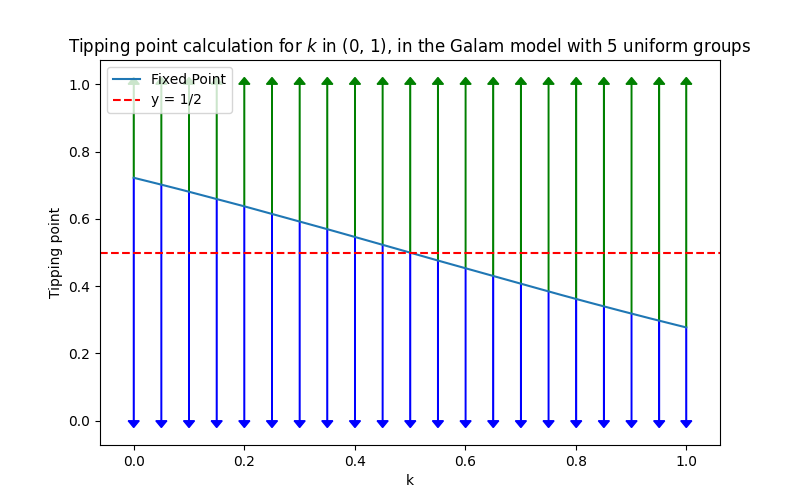
\includegraphics[width=\textwidth]{a515.png}
        \caption{Prevojne točke Galamovega modela s petimi enakomerno porazdeljenimi skupinami za različne vrednosti $k$.}
        \label{fig:a515}
    \end{subfigure}
    % Slika 2
    % Napis:Prevojne točke Galamovega modela s šestimi enakomerno porazdeljenimi skupinami za različne vrednosti $k$.
    % Datoteka: a616.png
    % Oznaka: fig:a616
    \begin{subfigure}{0.4\textwidth}
        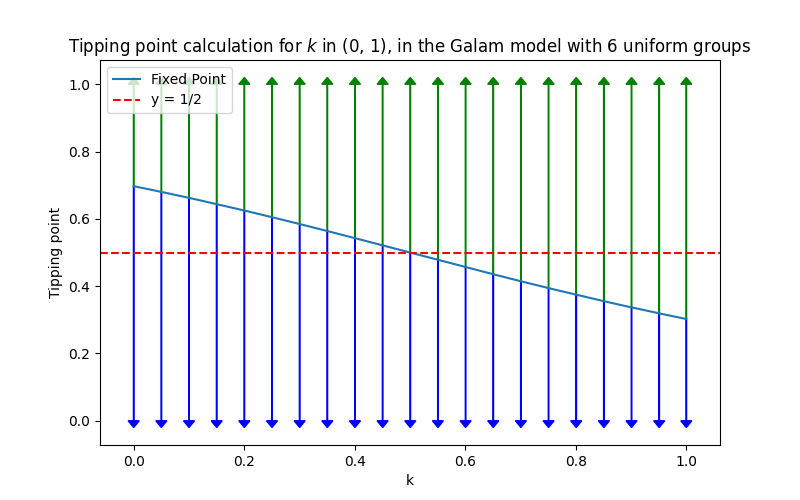
\includegraphics[width=\textwidth]{a616.png}
        \caption{Prevojne točke Galamovega modela s šestimi enakomerno porazdeljenimi skupinami za različne vrednosti $k$.}
        \label{fig:a616}
    \end{subfigure}
\end{figure}
% Literatura
\bibliographystyle{plain}
\bibliography{viri.bib}

\end{document}